\subsection{Research Questions}

The pre-project started by asking the following research question:
\begin{quote}
\textit{How can we modernize Model-Driven Development Frameworks to appeal to
the next generation of software developers, using recent developments in cloud
IDEs?}~\cite[p.~3]{rekstadModelingEnvironmentCloud2020}
\end{quote}

After answering this question, the pre-project narrowed down to the following research question:

\begin{quote}
\textit{How can we design an Ecore master-detail tree editor that works in both VSCode and Theia, while reusing existing tools for Ecore such as codegen and validation?}~\cite[p.~24]{rekstadModelingEnvironmentCloud2020}
\end{quote}

A set of five related sub-questions were also posed, and subsequently answered.
These questions set the context for a solution, and the stakeholders, constraints and requirements that would be needed.
The following subsections (\ref{subsec:stakeholders} to \ref{subsec:pre-project-protocol}) will present the results of the pre-project that are the basis of work done in this thesis.

\subsection{Stakeholders}\label{subsec:stakeholders}

A stakeholder is someone affected by or interested in the solution.
It can be an organization or people~\cite[p.~52]{bassSoftwareArchitecturePractice2013}.
The pre-project identified the key stakeholders in \cite[p.~3]{rekstadModelingEnvironmentCloud2020} to be:

%TODO use a table?
\begin{itemize}
  \item Kristian Rekstad (author). Goal: increase adoption of \acrshort{MDD} by students and industry. Has to design and develop the initial solution.
  \item Hallvard Trætteberg (supervisor). Goal: teach students the concepts of \acrshort{MDD} in \gls{TDT4250}. Wants to use \gls{Gitpod} and \acrshort{EMF} for student assignments.
  \item Teachers/Lecturers that use \acrshort{EMF}. Goal: teach students. Have to present the tree editor, use it and support students that ask for help.
  \item Students. Goal: learn useful technologies and pass courses like \gls{TDT4250} to get a grade. Will have to use \acrshort{EMF} if they study Computer Science with the ``Software Engineering'' specialization at \acrshort{NTNU}.
  \item Industry professional using \acrshort{EMF} to do \acrshort{MDD}. Goal: develop software for a business/client. May want to use \acrshort{EMF} without using \gls{Eclipse}, for personal reasons or organization policy.
  \item Eclipse Foundation. Goal: foster a community of developers and provide open source software. The maintainers of \acrshort{EMF}.
  \item Eclipse ecosystem developers. Goal: contribute to Eclipse Foundation projects. May possibly have to maintain and further develop this (or a derivative) solution if this project succeeds and they embrace it.
  \item Developers of third party \gls{VSCode} extensions that use tree editors. Goal: provide a high quality editor for their specific problem domain. Could use the architecture, protocol and frontends of this solution, if this solution is high enough quality, architected to be reusable and partially independent of \acrshort{EMF}, and reuse will reduce their design and/or development time.
\end{itemize}

\subsection{Software Requirements}

\paragraph{Requirement engineering approach}
The pre-project tried to establish the software requirements for a tree editor.
A literature review failed to find related works that listed the requirements for a tree editor.
The literature review also failed to find related works for modeling in the cloud with the purpose of creating \gls{Ecore} models.
The related works either \textit{deployed} \gls{Ecore} models to the cloud, were textual editors, or did not use \gls{Ecore}~\cite[p.~3]{rekstadModelingEnvironmentCloud2020}.\\

Without literature to suggest requirements, and without users to test on (except the author and supervisor), the best option was to analyze the existing tree editors in \gls{Eclipse}.
Common modeling tasks were performed (see \cref{par:tdt4250-confluence}), and detected functionality was recorded.
The result gave an initial list of functional requirements, but not a complete one.
However, by following an agile approach instead of waterfall, this list does not need to be complete\footnote{Agile values working software over extensive documentation, thus spending time on creating a working solution is better than a ``worthless'' list of everything a solution \textit{could have done}.}.
More requirements will emerge naturally as work progresses.
Still, having a good overview of the requirements is needed to correctly decide a software architecture, because of ``architecturally significant requirements'' that affect the architecture~\cite[p.~291]{bassSoftwareArchitecturePractice2013}.

\paragraph{Constraints}
A constraint is a restriction on the available choices for a solution~\cite[p.~7]{wiegersSoftwareRequirements2013}.
The most important constraint discovered was that the tree editor must be a \gls{VSCode} extension.
There is an alternative extension mechanism for \gls{Theia}, which was deemed incompatible with \gls{Gitpod}%
\footnote{Gitpod can use Theia as its editor frontend, but the user is not allowed to recompile and upload a new version of Theia. The alternative extension mechanism, \textit{Theia Extensions} needs a full recompilation of Theia~\cite[p.~38]{rekstadModelingEnvironmentCloud2020}. However, VSCode extensions can be installed during runtime, also in Theia in Gitpod.}%
~\cite[p.~38]{rekstadModelingEnvironmentCloud2020}.


\paragraph{Functional requirements}
A functional requirement specifies \textit{what} a solution must do, such as supported features~\cite[p.~7]{wiegersSoftwareRequirements2013}.
The pre-project identified several functional requirements for a tree editor in the cloud.
The full list of functional requirements, with id, requirement and description can be found in \cref{app:functional-requirements}.
The list can be summarized as follows:

\begin{itemize}
  \item Provide a master-detail tree editor in VSCode and Theia (Gitpod) by using an extension mechanism of the \gls{IDE}.
  \item The tree editor must show nodes with labels and icons as a hierarchy.
  \item Allow selecting a node in the tree editor by clicking it.
  \item Provide a property sheet for the selected node in the tree editor.
  \item Provide an action bar with actions that can be dynamically specified by a backend server.
  \item Child nodes can be hidden or shown in the tree by a user.
  \item The tree editor and property sheet must update when the underlying model changes in the server.
  \item The action bar shows appropriate actions based on the selected node.
  \item The tree editor must allow creation of new nodes.
  \item The tree editor must allow deleting nodes.
\end{itemize}

Some more important requirements were implicit, and not defined in the list.
This was not intentional, and an evidence to the list's non-completeness.
Some of the implicit requirements are explicitly defined as follows:

\begin{itemize}
  \item The editor must handle \gls{Ecore} models.
  \item The editor must handle model instances from \acrshort{XMI} files.
  \item The tree structure must be based on containment properties in the \gls{Ecore} model.
  \item The editor must provide a command in the \acrshort{IDE} to create a new \gls{Ecore} file with the minimum \acrshort{XMI} needed for a valid empty model.
  \item Tree nodes can be moved to new parents by drag-and-drop by the user.
  \item The drag-and-drop can not let the user drop a node on a parent that cannot contain the node as a child. 
  \item Saving a model will serialize it as \acrshort{XMI} to a file on disk.
  \item An action in the action bar must be added to run \textit{model validation}.
  \item An action in the action bar must be added to run \textit{code generation}.
  \item The editor shall show multiple tree roots when there are related model files. Opening a \gls{Ecore} file shall also show any genmodel file. A model instance shall also include a root for the \gls{Ecore} model in the same editor.
  \item A user can open more than one unique \gls{Ecore} model at the same time, in separate ``tabs'' in the editor.
  \item Any modification to the model must support undo and redo.
\end{itemize}


\paragraph{Non-functional requirements}
A non-functional requirement specifies characteristics or properties of the solution~\cite[p.~7]{wiegersSoftwareRequirements2013}.
Most of the non-functional requirements are grounded in empirical evidence like what the Eclipse ecosystem and web development ecosystems are currently doing.
A non-formal list of the non-functional requirements is as follows:

\begin{itemize}
  \item Compatibility with a code editor in \gls{Gitpod}.
  \item Use a permissive \gls{open source} license.
  \item Avoid software dependencies that are closed-source or use restrictive licenses.
  \item Use a distributed architecture with components reusable in other \acrshortpl{IDE}, inspired by architectures already in use by similar solutions~\cite[p.~24]{rekstadModelingEnvironmentCloud2020}.
  \item Configurability of user-facing options. Choices of colors, fonts, file system paths and similar should be possible to change~\cite[p.~24]{rekstadModelingEnvironmentCloud2020}.
  \item Configurability of mapping of \gls{Ecore} models to trees. Which containment references to use as children, and custom logic for labels should be user-specifiable~\cite[p.~24]{rekstadModelingEnvironmentCloud2020}.
  \item Localize the user interface in English.
  \item Flexibility and extensibility in the protocol to the server, allowing custom messages~\cite[p.~24]{rekstadModelingEnvironmentCloud2020}.
\end{itemize}


\subsection{Architecture and Protocol for a Solution}\label{subsec:pre-project-protocol}

A specific software architecture was proposed.
It had a goal to solve the requirements for: software reuse, \gls{Theia} and \gls{VSCode} compatibility, tree hierarchy editing, and a solution that could be transferable to other tree domains and editors.
Additionally, the protocol would try to stay close to related solutions, as they are empirically tested and familiar to developers in the Eclipse ecosystem.
By creating prototypes, major ``blockers'' or risk factors of the proposed architecture was tested and proven non-problematic~\cite[p.~38-46]{rekstadModelingEnvironmentCloud2020}.


\subsubsection{Architecture}

The tree editor shall be a \gls{VSCode} extension, and use the available \acrlongpl{API} for \gls{VSCode} extensions.
No dependencies to \gls{Theia} shall be introduced.
To view the tree structure as a hierarchy, the \textit{Custom Editor API} in \gls{VSCode} must be used (see \cref{sec:vscode-custom-editor}).
A custom editor can present the editor inside \gls{VSCode} as a \textit{WebView}, meaning a custom webpage free to render anything, isolated from the rest of \gls{VSCode}.


\paragraph{Components}
The editor thus comprises 4 components: the tree editor WebView (``\textbf{editor frontend}''), the \gls{VSCode} extension integration (``\textbf{extension}''), a \textit{Tree Language Server} (``\textbf{TLS}'') and the \textit{EMF.Cloud ModelServer} (``\textbf{ModelServer}'')~\cite[p.~48,49]{rekstadModelingEnvironmentCloud2020}.
An illustration is shown in \cref{fig:pre-project-tree-editor-architecture}

\begin{figure}[htbp]
  \centering
  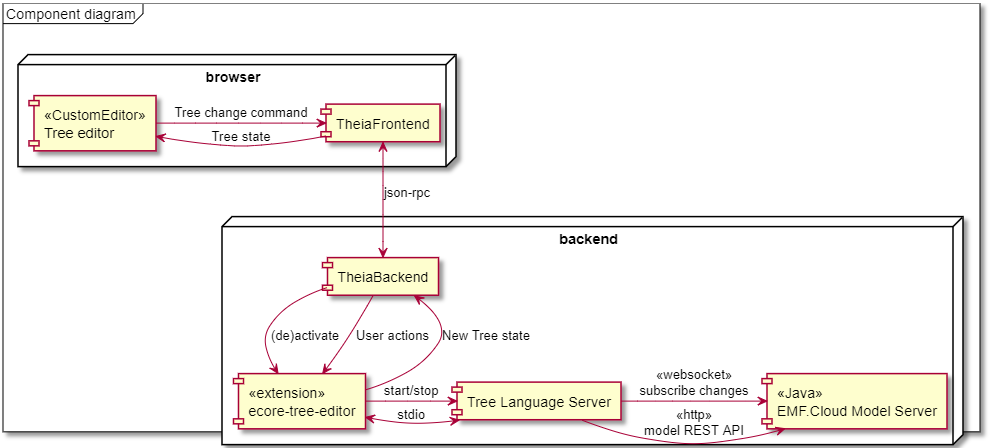
\includegraphics[width=\textwidth]{figures/pre-project/tree-editor-component-diagram.png}
  \caption[Tree Editor Architecture]{A suggested architecture for a tree editor. Copied from Figure 5.15~\cite[p.~49]{rekstadModelingEnvironmentCloud2020}. The diagram is based on \gls{Theia}, and the \gls{JSON-RPC} between TheiaFrontend and TheiaBackend happens behind the scenes, and is therefore not relevant to discuss.}\label{fig:pre-project-tree-editor-architecture}
\end{figure}


\paragraph{Editor frontend}
The editor frontend must be a web application that renders the tree as HTML, and provides interactivity with javascript. 
It communicates to the extension using \textit{messages} containing \gls{JSON}\footnote{This is a constraint imposed by the WebView API in VSCode.}.
The editor frontend will send messages that are \textit{commands} with the changes or actions a user triggered.
The extension will send messages with the new tree state to be shown.

\paragraph{Extension}
The extension is the main artifact which a user will install into \gls{VSCode} or \gls{Theia}.
This must be implemented with the \gls{TypeScript} language or javascript.
The extension will bundle the compiled code for the editor frontend, TLS and ModelServer inside it.
The extension is responsible for integrating with the \gls{IDE}, so that model files are opened in the custom editor, and handles commands triggered by the user in the \gls{IDE} (such as actions to create a new file, or saving a model).
The extension will start and stop the TLS process, and communicate over a \gls{JSON-RPC} protocol or \gls{REST} plus \gls{WebSocket}.
The extension and TLS can either use TCP sockets or standard in/out as the transport.

\paragraph{TLS}
A Tree Language Server (TLS) will contain specific knowledge about \gls{Ecore} and \acrshort{EMF}.
The choice of programming language is unconstrained.
The main purpose of the TLS is informing the extension of tree state, provide configuration for the tree editor and extension, and receive commands to modify models.
The TLS must be able to communicate using the same protocol as the extension (\gls{JSON-RPC} or \gls{REST} and \gls{WebSocket}), and either do so over standard in/out, or listen to incoming TCP sockets.
The TLS will perform commands to modify \acrshort{EMF} models by using as much re-use of existing code and frameworks as possible.
The TLS will start the ModelServer and communicate with it to read and modify models.
The ModelServer is a main part in the strategy to re-use existing code.

\paragraph{ModelServer}
This is a component already made by EclipseSource in java.
The ModelServer exposes \gls{REST} endpoints for working with \acrshort{EMF} models, such as listing models, reading models, and changing models with the EMF Commands framework.
Changes to a model are exposed as \gls{WebSocket} endpoints which can be ``subscribed'' to.


\subsubsection{Protocol}
The communication between the extension and the TLS should follow a defined protocol.
The protocol will contain the data structures and message formats to send, the serialization standard to use for messages, and define any required order for messages.


\paragraph{Base protcol}
The pre-project did not progress far enough to formally define this protocol, and did not implement it (or an alternative) either.
However, it specified a starting point and some rules.
The protocol should draw inspiration from the \acrlong{LSP}, and use the ``Base Protocol'' defined in \acrshort{LSP} (see \cref{sec:base-protocol}).
The Base Protocol has two parts: a HTTP header section, and a \gls{JSON-RPC} content section~\cite[p.~17,18]{rekstadModelingEnvironmentCloud2020}.
The content section will specify the remote procedures to be called, and contain the responses with data, such as tree structures, success or failure status, and errors.


\paragraph{Data structures}
This protocol can use the data structures to contain generic tree structures, proposed in Code listing 5.3 in \cite[p.~43,44]{rekstadModelingEnvironmentCloud2020} (added as \cref{lst:prototype2-node-tree} in \cref{app:pre-project-tree-structure}).
The protocol can not contain any specific references to \acrshort{EMF}, except as values in the generic data structures.
The central properties in the tree strucure was \textit{name}, \textit{type}, \textit{id} and \textit{children}.
The \textit{type} would for \gls{Ecore} be one of for example: \textit{EClass}, \textit{EPackage}, \textit{EReference} and so on.\\

The action bar should be populated based on a ``action schema'' data structure (Code listing 5.4 and 5.5 in \cite[p.~45]{rekstadModelingEnvironmentCloud2020}, see \cref{lst:prototype2-action-list} and \cref{lst:prototype2-action-schema} respectively in \cref{app:pre-project-tree-structure}), passed from the TLS to the extension in the protocol.\\

The hierarchy should be constrained by using a ``hierarchy schema'' (Code listing 5.6 in \cite[p.~45]{rekstadModelingEnvironmentCloud2020}, see \cref{lst:prototype2-hierarchy-schema} in \cref{app:pre-project-tree-structure}).
This would whitelist the allowed children for a node based on the \textit{type} property.
This would be passed from the TLS to the extension.
